
%% aici facem tranzitie de la problema generala de ML
%% la probleme cu secvente temporale, markov stuff, dbn shit
%% adica HMM-uri :))

%% Markov models, Dynamic Bayesian Networks
\begin{frame}
  \frametitle{Probleme cu Secvențe Temporale (I)}
  \only<1>{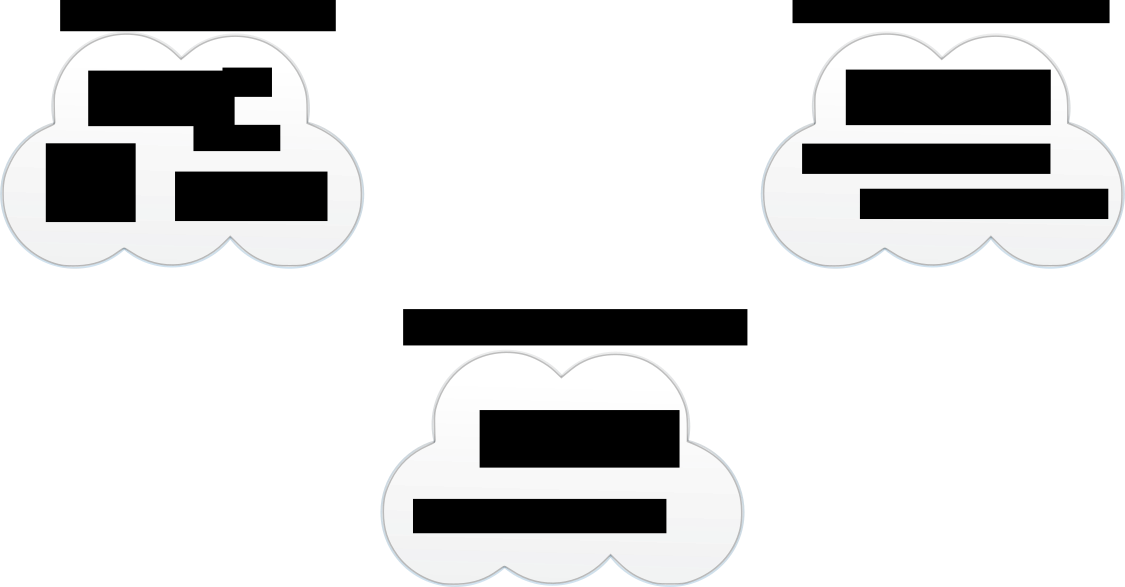
\includegraphics[width=\textwidth]{graphics/hmm-intro/time_series_problems_1.pdf}}
  \only<2>{
  	\includegraphics[width=\textwidth]{graphics/hmm-intro/time_series_problems_1_2.pdf}
  	\footnote{Sursa imaginii: Navstar}
  }
  \only<3>{
  	\includegraphics[width=\textwidth]{graphics/hmm-intro/time_series_problems_1_3.pdf}
  	\footnote{Sursa imaginii: http://www.hapblog.com/2012/01/iran-navy-tests-surface-to-air-missile.html}
  }
  \only<4>{
  	\includegraphics[width=\textwidth]{graphics/hmm-intro/time_series_problems_1_4.pdf}
  	\footnote{Sursa imaginii: http://www.redmondpie.com/}
  }
  \only<5>{
  	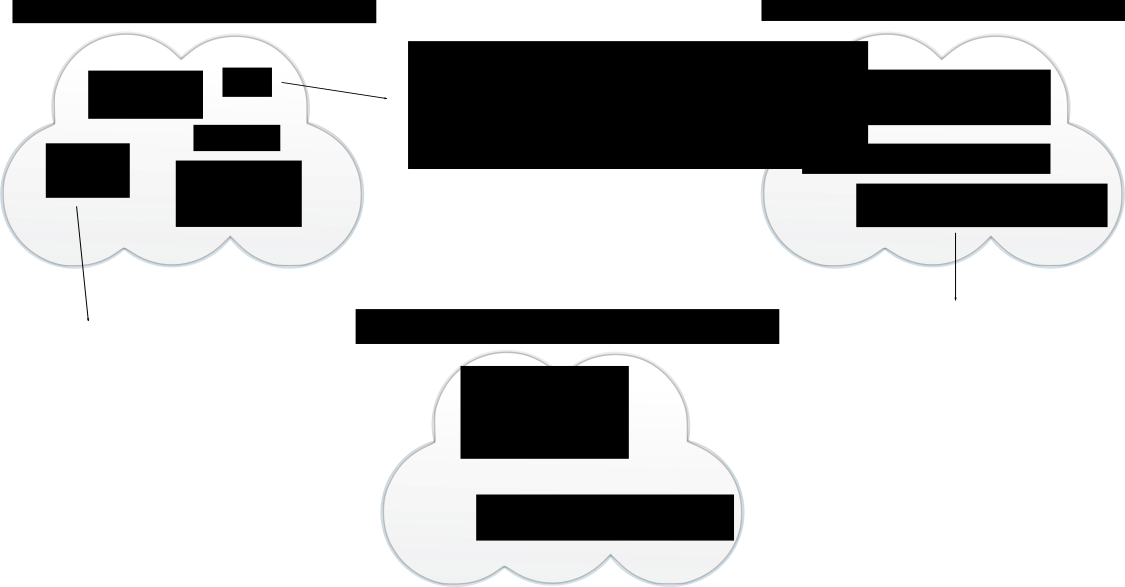
\includegraphics[width=\textwidth]{graphics/hmm-intro/time_series_problems_1_5.pdf}
  	\footnote{Sursa imaginii: http://desura.com}
  }
  \only<6>{
  	\includegraphics[width=\textwidth]{graphics/hmm-intro/time_series_problems_1_6.pdf}
  	\footnote{Sursa imaginii:  http://www.softpro.de}
  }
  
\end{frame}

\begin{frame}
  \frametitle{Probleme cu Secvențe Temporale (II)}
  \only<1>{
  	\includegraphics[width=\textwidth]{graphics/hmm-intro/time_series_problems_2.pdf}
  }
  \only<2>{
  	
\includegraphics[width=\textwidth]{graphics/hmm-intro/time_series_problems_2_2.pdf}
  	\footnote{Sursa imaginii:  http://www.econ.ucsb.edu/~doug/}
  }
\end{frame}


% descrierea a ceea ce inseamna Probabilistic Reasoning over Time (capitol 15.2 AI a modern approach)
% 	- states and observations
\begin{frame}[t]
  \frametitle{Raționament Probabilistic Temporal - Modele}
	
	Să ne gândim la unele din problemele anterioare ...	
	\vspace*{0.5em}
	\pause	
	
	Cum modelăm astfel de situații dinamice? 
	\vspace*{0.5em}
	\pause	
	
	\textbf{Stări și Observații}
	\begin{itemize}
		\item Procesul de schimbare este văzut ca o serie de \alert{snapshot-uri}
		\item Fiecare snapshot conține un set de variabile aleatoare
    	\begin{itemize}
			\item $\mathbf{O}_t$ - setul tuturor variabilelor de măsurare (\alert{\emph{observabile}}) la momentul \emph{t}
			\item $\mathbf{Q}_t$ - setul tuturor variabilelor de stare (\alert{\emph{neobservabile / ascunse}}) la momentul \emph{t}	    	
		\end{itemize}
	\end{itemize}
	
	\begin{figure}
		\centering
		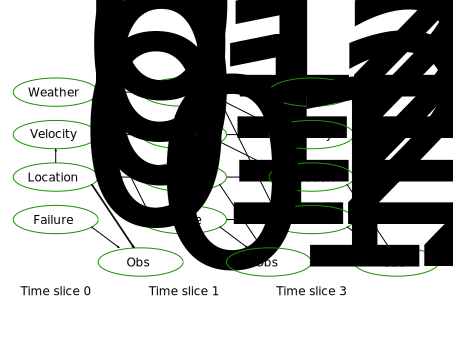
\includegraphics[height=0.3\textheight]{graphics/hmm-intro/dbn-vehicle/unrolled.pdf} 
  		\caption{\tiny{Exemplu: problemă de localizare a unui vehicul \citep{KollerFriedman09}}}
  		\label{fig:unrolled-states-observations}
  	\end{figure}
\end{frame}

%	- stationary process, Markov assumption, Sensor model
\begin{frame}[t]
  \frametitle{Raționament Probabilistic Temporal - Presupuneri}
	Să ne gândim la unele din problemele anterioare ...	
	\vspace*{0.5em}
	\pause	
	
	Ce \alert{presupuneri} (la o adică) facem?
	\pause	
	
	\begin{block}{Proces staționar}
		Procesul de schimbare este guvernat de legi care \alert{nu se schimba in timp}.\\
		\alert{Urmare:} trebuie sa specificăm relațiile între variabile doar pentru un snapshot \emph{reprezentativ}.	
	\end{block}
	\pause	
	
	\begin{block}{Presupunerea Markov}
		Starea curentă a unui proces de schimbare depinde doar de o \alert{istorie finită} de stări anterioare.\\
		\alert{Urmare:} avem un număr \alert{limitat} de ``parinți'' pentru variabilele din fiecare snapshot.
	\end{block}
  
\end{frame}

%	- inference in temporal models
%		- filtering
%		- prediction
%		- smoothing (hindsight)
%		- most likely explanation
%		- model learning
\begin{frame}
  \frametitle{Raționament Probabilistic Temporal - Inferență}
	Care sunt principalele inferențe ce se doresc făcute?	
	\pause	
	
	\begin{block}{Filtrare (monitorizare)}
		Sarcina de a calcula \alert{starea de fapt} - distribuția posterioară de probabilitate a 
		\alert{stării curente}, date fiind toate observațiile de până acum.
	\end{block}
	\pause
	
	\begin{block}{Evaluare}
		Sarcina de a calcula \alert{probabilitatea (likelihood)} a observațiilor făcute până în prezent.
	\end{block}  
\end{frame}

\begin{frame}
  \frametitle{Raționament Probabilistic Temporal - Inferență}
	\begin{block}{Predicție}
		Sarcina de a calcula distribuția posterioară de probabilitate peste o \alert{stare viitoare}, 
		date fiind toate observațiile de până acum.
	\end{block}
	\pause
	
	\begin{block}{Netezire (hindsight)}
		Sarcina de a calcula distribuția posterioară de probabilitate peste o \alert{stare anterioară}, 
		date fiind toate observațiile de până acum.\\
		Furnizează o estimare mai buna asupra stării respective, decât a fost posibil la momentul respectiv.
	\end{block}
\end{frame}

\begin{frame}
  \frametitle{Raționament Probabilistic Temporal - Inferență}
	\begin{block}{Cea mai probabilă explicație}
		Dându-se o \emph{secvență de observații}, se cere găsirea \alert{celei mai probabile secvenței de stări}
		care a generat acele observații.
	\end{block}
	\pause
	
	\begin{block}{Învățare}
		Dându-se \emph{un set de secvențe de observații}, găsește o metodă de a învăța \alert{modelele} de
		\alert{tranziție} și \alert{senzoriale / de măsurare} pe baza acelor observații.
	\end{block}
\end{frame}

\begin{frame}[t]
    \frametitle{Raționament Probabilistic Temporal - Metode Cunoscute}
    
  	\begin{block}{Rețele Bayesiene Dinamice (RBD)}
  		O RBD este o rețea Bayesiană ce reprezintă un model temporal de probabilitate.
  	\end{block}
  	
  	\begin{figure}
  		\centering
		\begin{subfigure}[b]{0.15\textwidth}
			\centering
  			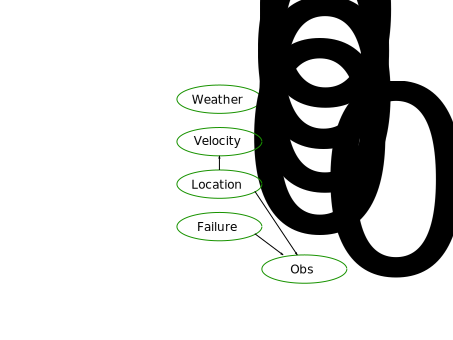
\includegraphics[width=\textwidth]{graphics/hmm-intro/dbn-vehicle/zero.pdf}
  			\caption{\tiny{Rețeaua Bayesiană în două snapshot-uri}}
  			\label{fig:2TBN}
  		\end{subfigure}
  		\begin{subfigure}[b]{0.30\textwidth}
			\centering
			\includegraphics[width=\textwidth]{graphics/hmm-intro/dbn-vehicle/transition.pdf}
  			\caption{\tiny{Rețeaua la momentul 0}}
  			\label{fig:zeroDBN}
  		\end{subfigure}
  		\begin{subfigure}[b]{0.35\textwidth}
			\centering
			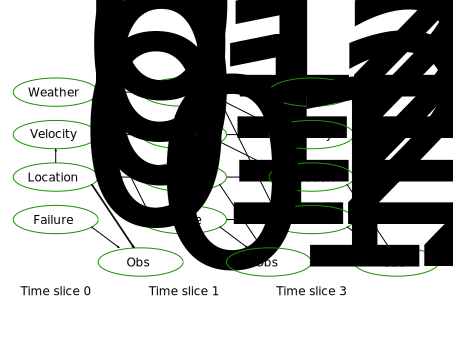
\includegraphics[width=\textwidth]{graphics/hmm-intro/dbn-vehicle/unrolled.pdf} 
  			\caption{\tiny{RBD desfășurată pe 3 momente de timp}}
  			\label{fig:unrolledDBN}
  		\end{subfigure}
  		\caption{\tiny{RBD simplificată pentru monitorizarea unui vehicul \citep{KollerFriedman09}}}
  		\label{fig:DBN}
  	\end{figure}
  	
  	\small{Aplicată în probleme precum: urmărirea obiectelor, recunoașterea activității umane, secvențierea proteinelor, etc.}
\end{frame}


\begin{frame}[t]
    \frametitle{Raționament Probabilistic Temporal - Metode Cunoscute}
  
  \begin{block}{Filtre Kalman (Sistem Dinamice Lineare)}
	Un model temporal având una sau mai multe variabile care evoluează linear în timp, la care se adaugă 
	\alert{zgomot Gaussian}.
  \end{block}
  
  \begin{columns}[T]
  	\column{0.4\textwidth}
  	\begin{figure}
  		\centering
  		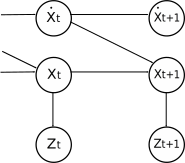
\includegraphics[height=0.35\textheight]{graphics/hmm-intro/kalman/kalman_filter_simple.pdf}
  		\caption{\tiny{Structura unei RB pentru un sistem linear dinamic cu variabile de poziție $X_t$, 
  		viteză $\dot{X}_t$, și măsurare a poziției $Z_t$}}
  	\end{figure}
	  
  	\column{0.6\textwidth}
  	\begin{itemize}
  		\item \footnotesize{Poate fi văzut ca o RBD în care toate variabilele sunt continue, iar dependențele sunt 
  		linear gaussiane.}
  		\item \footnotesize{Aplicații multiple în \textbf{urmărirea obiectelor}}
  	\end{itemize}
  \end{columns}
  
\end{frame}

\begin{frame}[t]
    \frametitle{Raționament Probabilistic Temporal - Metode Cunoscute}
  
  \begin{block}{Modele Markov Ascunse (MMA)}
	Un MMA (HMM) este un model probabilistic temporal în care \emph{starea} procesului de schimbare este descrisă
	de \alert{o singură variabilă aleatoare discretă}.
	Valorile posibile ale variabilei reprezintă stările posibile ale lumii modelate.
  \end{block}
  
  \vspace*{1em}
  
  Utilizat cu succes in aplicații precum:
  \begin{itemize}
  	\item Recunoasțerea Scrisului
  	\item Recunoasțerea Gesturilor
  	\item Recunoasțerea Vorbirii
  	\item Determinarea Parților de Vorbire (Part-of-Speech Tagging)
  	\item Secvențiere ADN
  \end{itemize}
\end{frame}

